% --- Configuration ------------------------------------------------------
% add shortcut for github url of this chapter
\def \GITHUB {\GITHUBBASE/05_psychoacoustics}


% --- Document -----------------------------------------------------------
\chapter{Psychoacoustics of Sound Field Synthesis}
\label{cha:psychoacoustics}

\firstthought{The perception} of synthesized sound fields could be highly
affected by the errors that are introduced into the sound
field by practical setups, as discussed in
Chapter\,\ref{cha:sound_field_errors_and_their_perceptual_relevance}.
In this chapter, different experiments are presented that investigate
the influence of those errors on the perception and if an
authentic synthesis is possible at all. The investigation is split up in
single experiments for different perceptual attributes.
It will start with measuring the localization
accuracy as an indicator for spatial fidelity for \ac{WFS} and \ac{NFC-HOA} and
different secondary source distributions. This approach will be repeated for timbral
fidelity and \ac{WFS}.
The last section deals with the special case of focused sources in \ac{WFS} for
which spectro-temporal artifacts are another perceptual attribute in addition to
coloration and localization accuracy.


%%%%%%%%%%%%%%%%%%%%%%%%%%%%%%%%%%%%%%%%%%%%%%%%%%%%%%%%%%%%%%%%%%%%%%%%%%%%%%%%
\section[Spatial Fidelity]{Spatial Fidelity\autocite[Parts of this section are published
in][]{Wierstorf2012c,Wierstorf2013}}
\label{sec:localization}

The human auditory system has the remarkable ability to detect the horizontal
direction of a sound source up to a accuracy of $1\degree$. This imposes strict
requirements on a spatial audio system, if the system tries to achieve
authenticity
compared with the real world. In this section the localization accuracy of the
listener for different sound field synthesis systems is investigated in a
systematic way. It is shown which distance of the loudspeakers is required to
achieve authenticity and what happens for larger inter-loudspeaker
distances. In the next step, the properties of the
synthesized sound fields that allow or hinder the localization will be discussed.

For the simplest possible spatial audio system -- the stereophonic setup -- it is
well known that the localization is only correct inside a small area which is
called the sweet-spot. If the listener is standing outside the sweet-spot, the
localization is dominated by the position of the nearest loudspeaker.
For sound field synthesis methods, on the other hand, it is assumed that they are
able to provide an equally good localization in the whole listening area. A
feature that is especially claimed for \ac{WFS}.
But a transition from the sweet-spot-like behavior of stereophony to
sound field synthesis has to take place for \ac{SFS} setups applying a low
number of loudspeakers. A good
example is band-pass limited \ac{NFC-HOA}, for which also a pronounced sweet-spot
exists in the center of the loudspeaker array -- compare
Figure\,\ref{fig:nfchoa_aliasing}.

Localization was investigated for different sound field synthesis setups in the
last years, but in most of the publications only a central
listening position was considered.

Test results for \ac{WFS} show that the
localization
at a central listening position is not or only slightly impaired
for loudspeaker spacings less than
$25$\,cm.\autocite{Vogel1993,Start1997,Wittek2007}
All studies included a synthesized point source and different linear
loudspeaker arrays.
The experiments were performed directly with a localization test or indirectly with a
minimum audible angle experiment\autocite{Vogel1993}. No differences were found
between the results for
broadband stimuli and low-pass stimuli, containing only energy below the
aliasing frequency. This indicates that the distortions for
\acp{ITD} and \acp{ILD} at high frequencies due to the spatial aliasing artifacts
apparently does not influence the localization accuracy.
Verheijen has carried out localization tests for point sources and focused sources
placed at different positions.\autocite{Verheijen1997}
For a loudspeaker spacing of $11$\,cm he found no difference in localization 
compared to a real source. For a spacing of $22$\,cm the localization blur
increased by $0.5\degree$.
If an infinitely long linear array is applied, the localization impact due to a
change of the source position would be equivalent to that due to the change of the listener
position. The length of the array in Verheijen's experiment was $2.53$\,m, which
is too short to apply this equivalence.

For \ac{NFC-HOA} no localization results are available. For \ac{HOA} experiments
were carried out for a central and in some cases one off-center listening
position.\autocite[E.g.][]{Bertet2013}
In all of the studies a maximum Ambisonics order of five was investigated.
Systems with low orders like these are more
equivalent to stereophonic panning approaches than sound field synthesis
methods. This implies that for off-center listening positions the synthesized
source will be localized towards the nearest loudspeaker -- compare Figure\,7 in
Spors et al.\autocite{Spors2013a}
For the highest order of five the localization was no longer strictly bound
to the nearest loudspeaker and a localization accuracy around
$3\degree$ could be achieved.\autocite{Frank2008}

In this thesis, the focus of the localization experiments lies on two aspects.
At first, the accuracy in the whole audience area should be assessed. This was ensured
by applying 16 different listener positions, equally distributed in the
audience area. In addition, the dependence of the localization accuracy on the
distance between adjacent loudspeakers was investigated. To achieve this,
three different loudspeaker distances were tested for a linear and a circular
loudspeaker array. For \ac{NFC-HOA} another dependency was added by varying the order
of the spherical harmonics using the same loudspeaker distance.

The tests were split in four different experiments, which will be introduced
in the following.


%--%--%--%--%--%--%--%--%--%--%--%--%--%--%--%--%--%--%--%--%--%--%--%--%--%--%-
\subsection{Method}
\label{sec:localization_method}
%
The different loudspeaker arrays were simulated via the dynamic binaural synthesis
system described in Section\,\ref{sec:experimental_setup_of_binaural_synthesis}.
The test procedure was the same as described in
Section\,\ref{sec:verifying_binaural_synthesis_for_localization_experiments},
including the pointing method, test setup, and white noise pulse.
That means that the listener listened to a binaural simulation of a sound
field synthesis system synthesizing a white noise pulse. Thereafter, the
listener was to
look into the direction from which she perceived the noise and press a key,
with the
laser pointer mounted on the headphones, providing her visual feedback about
her viewing direction.

In the
following, the different sound field synthesis conditions, loudspeaker setups, and
test participants will be described for every experiment.
The test participants were financially compensated for their effort. All of them
had self-reported normal hearing.
The presentation of the conditions was randomized, with the exception that -- due to
limited computing power -- all conditions belonging to one source model were
presented together. The order of the source models for every listener was again
randomized.


%----%----%----%----%----%----%----%----%----%----%----%----%----%----%----%----
\paragraph{Experiment 1: \ac{WFS}, Linear Loudspeaker Array}
\label{sec:experiment1_wfs_linear_array}
%
\begin{marginfigure}
    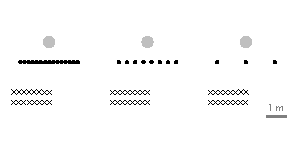
\includegraphics{fig5_01/fig5_01}
    \caption{Setup for Experiment 1. The position of the synthesized
    source is indicated by the grey point. The position of the listener by black
    crosses and secondary sources by black dots.
        \reproduce{\GITHUB/fig5_01}}
    \label{fig:setup_wfs_linear_array}
\end{marginfigure}
%
Three different linear loudspeaker setups were considered in the experiment. The
length of the loudspeaker array was always $2.85$\,m, measured from the center
of each edge loudspeaker. The center of the loudspeaker array was placed at
$(0,0,0)\,m$. The number of loudspeakers varied,
including 3, 8, and 15 loudspeakers. This corresponds to a distance of
adjacent loudspeakers of $1.43$\,m, $0.41$\,m, and $0.20$\,m. For each loudspeaker
setup a point source was synthesized at $(0,1,0)$\,m with \ac{WFS}
using \eqref{eq:d_wfs_ps_25D} to calculate the driving functions.

The listeners were placed at 16 different positions: $(0,-1.5,0)$\,m,
$(-0.25,-1.5,0)$\,m, $(-0.5,-1.5,0)$\,m, $(-0.75,-1.5,0)$\,m,
$(-1,-1.5,0)$\,m,
$(-1.25,-1.5,0)$\,m, $(-1.5,-1.5,0)$\,m, $(-1.75,-1.5,0)$\,m, $(0,-2,0)$\,m,
$(-0.25,-2,0)$\,m, $(-0.5,-2,0)$\,m, $(-0.75,-2,0)$\,m, $(-1,-2,0)$\,m,
\linebreak
$(-1.25,-2,0)$\,m, $(-1.5,-2,0)$\,m, $(-1.75,-2,0)$\,m  -- compare
Figure\ref{fig:setup_wfs_linear_array}.
Only positions in the left half of the listening area were considered due to the
symmetry of the problem.
Because everything was simulated via
binaural synthesis the listener was able to switch instantaneously between the
different positions -- see Chapter\,\ref{cha:binaural}.

Three different loudspeaker setups and 16 different listening positions
led to a total of 48 conditions, which were presented five times to every
listener. The listening experiment was split into two sessions to avoid fatigue:
one session for the listener positions with a $y$-position of $-1.5$\,m and
the other for a $y$-position of $-2$\,m. Additionally, each session
included ten presentations of a real loudspeaker at an azimuth of
$-5.7\degree$.
For the array with 8 loudspeakers the test participant's viewpoint in the simulation
was rotated by $35\degree$, and for the array with 15 speakers by $17.5\degree$.
This was done to ensure
an evenly distribution of the virtual source positions to the left/right of the
listener.

11 listeners were recruited for the experiment -- aged 21 to 33 years.
Four of them had prior experiences with psychoacoustic testing and \ac{WFS}.
One test participant was removed from the analysis, because the standard
deviation for the repeated conditions was approximately three times as high as
for the average listener.
% average = 2.29 +- 0.3
% VP07 = 6.18 +- 1.1


%----%----%----%----%----%----%----%----%----%----%----%----%----%----%----%----
\paragraph{Experiment 2: \ac{WFS}, Circular Loudspeaker Array}
\label{sec:experiment2_wfs_circular_array}
%
\begin{marginfigure}
    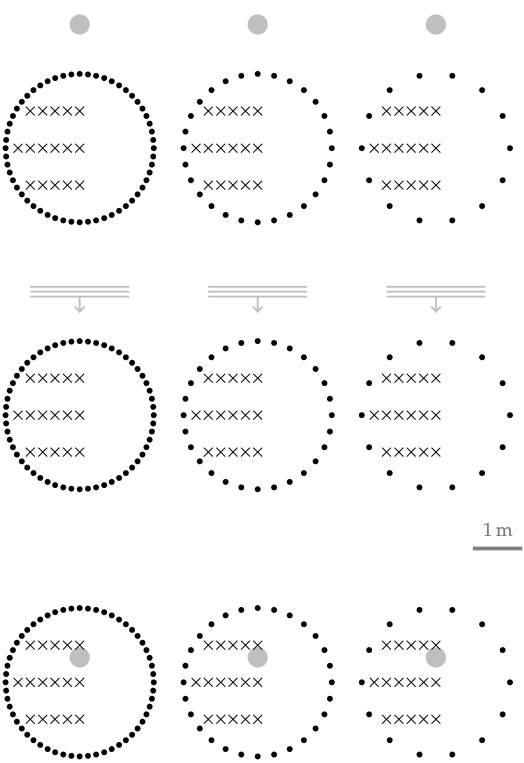
\includegraphics{fig5_02/fig5_02}
    \caption{Setup for Experiment 2. The position of the synthesized
    source is indicated by the grey point. The position of the listener by black
    crosses and secondary sources by black dots.
        \reproduce{\GITHUB/fig5_02}}
    \label{fig:setup_wfs_circular_array}
\end{marginfigure}
%
The experiment consisted of three different circular loudspeaker setups. The
diameter of the loudspeaker array was $3$\,m. The center of the
loudspeaker array was placed at $(0,0,0)$\,m. The number of loudspeakers
varied between 14, 28, and 56 loudspeakers. This corresponds to a distance
of adjacent loudspeakers of $0.67$\,m, $0.34$\,m, $0.17$\,m.
For every loudspeaker setup a point source placed at $(0,2.5,0)$\,m, a plane wave
traveling into the direction $(0,-1,0)$, and a focused source placed at $(0,0.5,0)$\,m
were synthesized with \ac{WFS} using \eqref{eq:d_wfs_ps_25D}, \eqref{eq:d_wfs_pw_25D}
and \eqref{eq:d_wfs_fs_25D} to calculate the driving functions.

The test participants were placed at 16 different positions: \linebreak
$(0,0.75,0)$\,m,
$(-0.25,0.75,0)$\,m, $(-0.5,0.75,0)$\,m $(-0.75,0.75,0)$\,m, \linebreak
$(-1,0.75,0)$\,m,
$(0,0,0)$\,m, $(-0.25,0,0)$\,m, $(-0.5,0,0)$\,m, $(-0.75,0,0)$\,m $(-1,0,0)$\,m,
$(-1.25,0,0)$\,m, $(0,-0.75,0)$\,m, $(-0.25,-0.75,0)$\,m, \linebreak
$(-0.5,-0.75,0)$\,m,
$(-0.75,-0.75,0)$\,m, $(-1,-0.75,0)$\,m -- compare
Figure\,\ref{fig:localization_results}.

Three different loudspeaker setups, 16 different listening positions, and
three different source types resulted in a total of 144 conditions, which were
presented five times to every listener. The measurement was split up in two
days, one session lasted approximately 45 minutes.

To ensure a more equal distribution of the presented locations of the sound
events a pseudo-randomized jitter was added to the listener's viewpoint.
They were chosen in a way that the position of the sound event always was within
the boundary of $\pm 30\degree$.

12 listeners were recruited for the experiment -- aged 23 to 33 years.
One of them had prior experiences with psychoacoustic testing and \ac{WFS}.


%----%----%----%----%----%----%----%----%----%----%----%----%----%----%----%----
\paragraph{Experiment 3: \ac{NFC-HOA}, Circular Loudspeaker Array}
\label{sec:experiment3_nfchoa_circular_array}
%
\begin{marginfigure}
    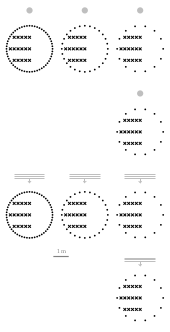
\includegraphics{fig5_03/fig5_03}
    \caption{Setup for Experiment 3. The position of the synthesized
    source is indicated by the grey point. The position of the listener by black
    crosses and secondary sources by black dots.
        \reproduce{\GITHUB/fig5_03}}
    \label{fig:setup_hoa_circular_array}
\end{marginfigure}
%
Here, the same circular loudspeaker setups and listening positions as described for
Experiment 2 were applied. For every loudspeaker setup a point source placed at
$(0,2.5,0)$\,m and a plane wave traveling into the direction
$(0,-1,0)$ were synthesized with band-limited \ac{NFC-HOA} using
\eqref{eq:D_nfchoa_ps_25D} and
\eqref{eq:D_nfchoa_pw_25D} to calculate the driving functions. The time domain
implementations of the driving functions were realized as filters.
For the loudspeaker setup with 14 loudspeakers, both sources were
also synthesized with \ac{NFC-HOA} using an order of $M = 28$.

Four different loudspeaker setups and orders of spherical harmonics
combinations, 16 different listening positions, and two different source types
resulted in a total number of 128 conditions, which were presented five times to
every listener. The measurement was split up in two days, one session lasted
approximately 40 minutes.

The positions of the sound events were again jittered as described for
Experiment~2.

A pre-test showed that the synthesis of one point source or one plane wave
could lead to two auditory events coming from different directions that could be
quite far away from each other. Therefore, in this experiment it could not be
assured for all conditions that the auditory event was perceived in a region $\pm
30\degree$. This is important, because the pointing method has some
deviations for angles outside of this region -- compare
Figure\,\ref{fig:binaural_synthesis_localization}.
In addition, the instruction for the test participants were slightly updated and
they were told to look into the direction of the more pronounced source,
if they heard more than one. In cases where they were not able to state which
was
more pronounced, they were instructed to randomly choose one of the sources.

12 listeners were recruited for the experiment -- aged 24 to 35 years.
Three of them had prior experience with psychoacoustic testing and sound field
synthesis.
One of the listeners completed only the condition with plane wave as source
model and one completed only the condition with point source as source model.
Two test participants were excluded from the analysis, because their standard deviation
for the five repetitions was more than twice as large as for the other
participants.


%----%----%----%----%----%----%----%----%----%----%----%----%----%----%----%----
\paragraph{Experiment 4: \ac{NFC-HOA}, Number of Sources}
\label{sec:experiment4_nfchoa_circular_loudspeaker_array_number_of_sources}
%
Due to the fact that for some conditions in Experiment 3 more than one auditory
event was audible, a post-test was conducted. The listeners were asked to
indicate on a keyboard how many sources they heard: one or two?
The same conditions as in Experiment 3 were used, but this time each condition
was only repeated four times.
All conditions were presented in one session lasting approximately 40 minutes.

7 listeners were recruited for the experiment -- aged 23 to 33 years.
Three of them had prior experience with psychoacoustic testing and sound field
synthesis.




%--%--%--%--%--%--%--%--%--%--%--%--%--%--%--%--%--%--%--%--%--%--%--%--%--%--%-
\subsection{Results}
\label{sec:localization_results}
%
\begin{figure}
    \centering
    \hspace*{-1.2cm}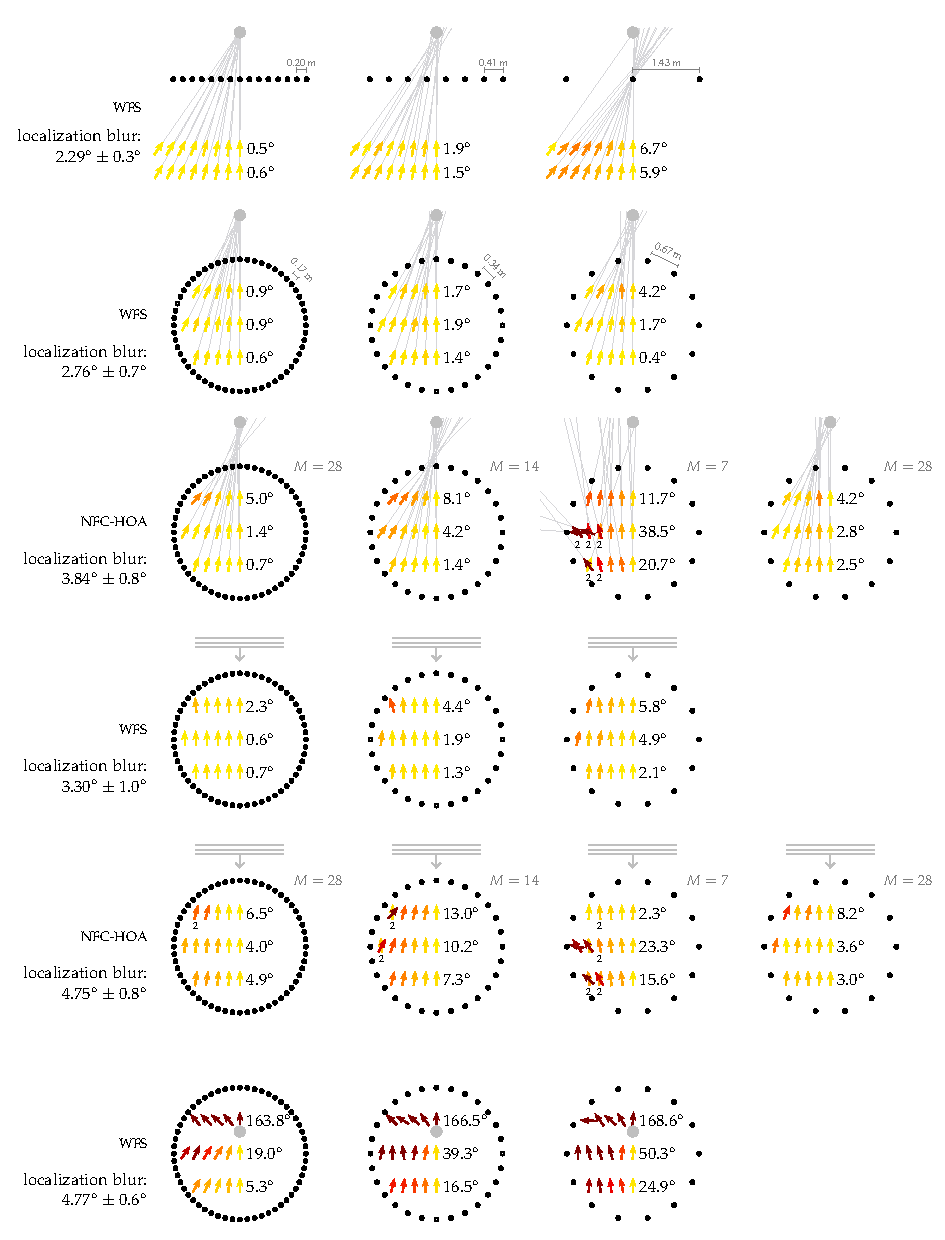
\includegraphics{fig5_04/fig5_04}
    \caption{Average localization results for all four experiments. The black
    symbols indicate loudspeakers, the grey ones the synthesized source. At
    every listening position, an arrow is pointing into the direction from which the
    listeners perceived the corresponding auditory event. The color of the arrow
    displays the absolute localization error, which is also summarized as an
    average beside the arrows for every row of positions. The average confidence interval for
    all localization results is $2.3\degree$. Listening conditions which
    resulted in listeners saying that they perceived two sources in Exp.\,4 are
    highlighted with a small $2$ written below the position.
        \reproduce{\GITHUB/fig5_04}
    }
    \label{fig:localization_results}
\end{figure}
%
Figure\,\ref{fig:localization_results} summarizes the results of all four
experiments. For every sound field synthesis method, the used loudspeaker setups
are drawn as black dots and the synthesized sources are indicated by the grey
symbols. At every listener position an arrow is pointing towards the average direction
from which the listeners perceived the corresponding auditory event. The added random jitter
of the head orientation of the listener at every position is already compensated
in the presented arrows. The color of each arrow displays the localization
error, which is defined as the absolute deviation between the desired sound
event direction and the direction of the auditory event. The absolute deviation
is represented by the color, ranging from light yellow for $0\degree$ to dark red
for values of $40\degree$ or higher.
For the
condition of the synthesized point source, the perceived direction of the listener is
additionally highlighted by a small grey line going into this direction.
The results from the fourth experiment, where no direction but only the number
of perceived sources is the outcome, are included by adding a small ``2'' below the
position of all conditions where two sources were perceived. For no condition
more then two sources were perceived.

The localization error for \ac{WFS} synthesizing a point source or a plane wave
is approximately $0.9\degree$ in the case of loudspeaker spacings around
$20$\,cm. Only the position $(-1,0.75,0)$\,m for the synthesis of a plane wave
deviates from this pattern and yielded an error of around $5\degree$. For the synthesis
of a plane wave with \ac{WFS} the dependency of the localization error on the
position is more pronounced for larger loudspeaker spacings. Here,
especially the positions to the side near the loudspeakers lead to larger
localization errors than in the case of the point source conditions. For a
loudspeaker spacing around $40$\,cm the localization error increases only slightly
to an average of $2\degree$. For larger loudspeaker spacings the
localization error increases and varies for different listening
positions. In addition, the listeners start to look into the direction of the
nearest loudspeaker instead of the direction of the synthesized point source.
This is most prominent for the linear loudspeaker array with only three
loudspeakers and a loudspeaker spacing of $1.43$\,m.

The localization error for band-limited \ac{NFC-HOA} synthesizing the same
point source is larger at all positions, starting at $3.8\degree$ for a
loudspeaker spacing of $17$\,cm and $7.4\degree$ for a spacing of $34$\,cm.
The results are more dependent on the listening position as for the \ac{WFS}
conditions, showing stronger errors for positions to the side.
In the case of the loudspeaker array with 14 loudspeakers, the
localization error for the point source condition is larger than $10\degree$ for
most of the positions to the side. In addition, for five positions to the side
the listeners reported that they heard more than one auditory event.

For the case of a loudspeaker array with 14 loudspeakers, \ac{NFC-HOA}
up to an order of $M = 28$ was also tested. An order of $28$
corresponds the order of band-limited
\ac{NFC-HOA} for the loudspeaker array with 56 loudspeakers. 
In this case, the results are very similar to the ones of the \ac{WFS} conditions
for 14 loudspeakers. The overall localization error is slightly larger than for
\ac{WFS}. In contrast the pattern is very similar for the point source as well as for the
plane wave conditions, meaning that the localization error now has similar
values for all positions across the listening area
and only one auditory event is perceived at all
positions.

\begin{figure}
    \centering
    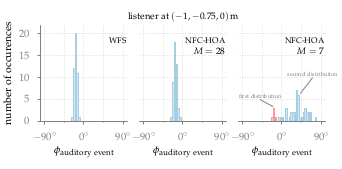
\includegraphics{fig5_05/fig5_05}
    \caption{Distributions of the directions of the auditory event as rated by
    the listeners at the position $(-1,-0.75,0)$\,m for the loudspeaker array with
    14 loudspeakers. The results for a synthesized point source for \ac{WFS} and
    \ac{NFC-HOA} for different orders $M$ are shown. For \ac{WFS} only the
    results for the first 9 listeners were analyzed to have an equal number of
    answers as in the case for \ac{NFC-HOA}.
        \reproduce{\GITHUB/fig5_05}
    }
    \label{fig:localization_distribution}
\end{figure}
%
\newthought{In order to} analyze the influence of more than one auditory event on the
localization ratings, the distributions of the reported directions of auditory
events from all listeners were visually proofed for normal distribution. An
example is presented in Figure\,\ref{fig:localization_distribution} for the point
source condition at the listening position $(-1,-0.75,0)$\,m. The distributions
of ratings of 9 listeners are shown in comparison for \ac{WFS} and \ac{NFC-HOA}
with an order of $28$ and of $7$. For the case of \ac{WFS} and \ac{NFC-HOA} with an
order of $28$, a normal distribution is visible. On the other hand, for the case
of \ac{NFC-HOA} with an order of $7$ the distribution is far more spread and the
data are most probably characterized by more than one normal distribution. In all
cases where visual inspection leads to the assumption of two underlying normal
distributions, a Gaussian mixture model was applied to estimate what data point
belongs to what distribution. This was repeated for 100 iterations for each
position. Afterwards the data points were assigned to their belonging average.
The two distributions and their corresponding data points are
indicated by two different colors in
Figure\,\ref{fig:localization_distribution}. After the assignment to a particular
distribution, the average direction was calculated for every distribution. In
Figure\,\ref{fig:localization_results} two arrows, one for each corresponding
direction were drawn for all positions where more than one normal distribution
was found.

\newthought{For WFS}, the localization of focused
sources placed in the audience area is investigated in the following.
The results are shown
at the bottom row of Figure\,\ref{fig:localization_results}. The focused source
was placed at $(0,0.5,0)$\,m and was heading towards $(0,-1,0$)\,m, which means that
the five listener positions with $y=0.75$\,m were placed between the focused
source and the active loudspeakers. For these positions, the listeners were not
looking into the direction of the focused source but into the direction of the
active loudspeakers, which leads to large localization errors, because the
loudspeakers are up to $180\degree$ opposite of the focused source direction.
In addition, it could be observed that for the loudspeaker arrays with 14 and 28
loudspeakers only a small region with low localization error exists around the
central listening positions. For positions to the side, the
listeners were again pointing more into the direction of the active loudspeakers.
Only for the loudspeaker array with $17$\,cm spacing
between the loudspeakers, a triangle-shaped listening area can be identified where the
localization error is around or less than $10\degree$.


%--%--%--%--%--%--%--%--%--%--%--%--%--%--%--%--%--%--%--%--%--%--%--%--%--%--%-
\subsection{Discussion}
\label{sec:localization_discussion}
%
The ability to localize a sound that is synthesized by \ac{WFS} is very good in
the whole audience area, independent of the form of the secondary sources. The
localization error for a synthesized point source and a synthesized plane wave
is below $5\degree$ on average and is only degraded for positions in the
proximity of around $20$\,cm to the loudspeakers. Only if a small number of loudspeakers
is employed, the localization error will become the same as for the case
of stereophony, meaning that the direction of a single loudspeaker rather than of
the desired source will be perceived. This was the case for the linear
loudspeaker array with 3 loudspeakers in the presented tests.

The localization accuracy for the same secondary source setups driven by
band-limited \ac{NFC-HOA} is inferior to that of \ac{WFS}. Only the secondary source
distribution employing 56 sources is capable of providing a localization error
smaller than $5\degree$ in most of the audience area. For fewer secondary
sources, large localization errors occur outside the center of the audience
area. In the case of 14 sources, the listeners start to perceive more than one
source and hear single loudspeakers.
If in the case of 14 sources the order of \ac{NFC-HOA} is chosen not to be
band-limited to $7$, but going up to $28$ as it would be the case for 56
sources, the localization accuracy is comparable to that of band-limited
\ac{NFC-HOA} with the same order and 56 sources. This highlights that in the
case of \ac{NFC-HOA} the applied order is very critical for the localization
accuracy in the whole audience area. If the order is reasonably high,
localization performance will be identical to hat of \ac{WFS}. Otherwise it will be
impaired outside of the center of the audience area.
This is not surprising, remembering Figure\,\ref{fig:sound_field_imp} where the
impulse responses of different \ac{SFS} systems were shown. \ac{WFS} and
\ac{NFC-HOA} behave similarly if the order of \ac{NFC-HOA} is high enough,
in opposition to the splitting of the impulse for different frequency regions
outside of the center for band-limited
\ac{NFC-HOA} -- compare also Figure\,\ref{fig:sound_field_imp_fixed_filtered}.

By comparing the localization blur it can be seen that for \ac{NFC-HOA} the
synthesized sources will be perceived on average to have a slightly larger spatial
extent than for \ac{WFS}.

\newthought{For the special case} of the synthesis of a focused source with
\ac{WFS}, the
localization accuracy depends strongly on the secondary source distribution. In
contrast to the case of a plane wave or point source, a synthesized focused
source achieves an extended listening area only for the setup with 56 sources.
The localization blur further indicates that focused sources are perceived to be
the widest synthesized sources in all of the experiments. This can be explained
by the fact that the size of the focal point is limited by the wavelength of the
sound, leading to a large focal point size especially for low frequencies.


%--%--%--%--%--%--%--%--%--%--%--%--%--%--%--%--%--%--%--%--%--%--%--%--%--%--%-
\subsection{Conclusion}
\label{sec:localization_conclusion}
%
If a sound field synthesis system is desired that is authentic with regard to the
localization accuracy, \ac{WFS} and a
distance between the loudspeakers of at least $20$\,cm can already lead to
satisfactory results.
If a larger distance of loudspeakers is applied, \ac{WFS} still leads to a very
high localization accuracy in the whole audience area. Especially in these cases
it can deliver a superior localization accuracy compared to band-limited
\ac{NFC-HOA} which has large localization errors outside of the sweet-spot.
Inside the sweet-spot the localization accuracy is authentic in terms of the
desired result as well.
But outside, more than one source could be perceived. 

If \ac{NFC-HOA} is desired for synthesis and good localization
accuracy should be achieved in the whole audience area, the Ambisonics order
should be increased to a reasonable number. In that case,
\ac{NFC-HOA} becomes comparable to \ac{WFS}, which constitutes a high-frequency
approximation of \ac{NFC-HOA} with infinite order.



%%%%%%%%%%%%%%%%%%%%%%%%%%%%%%%%%%%%%%%%%%%%%%%%%%%%%%%%%%%%%%%%%%%%%%%%%%%%%%%%
\section[Timbral Fidelity]{Timbral Fidelity\autocite[This experiment
was published in a slightly modified way in][the presented experiment was carried
out in coorperation with Christoph Hohnerlein as part of his Bachelor
thesis]{Wierstorf2014}}
\label{sec:timbral_fidelity}

Section\,\ref{sec:spatial_aliasing_and_discrete_secondary_source_distributions}
showed that a limited number of secondary sources leads to a repetition of parts
of the desired synthesized signal. In the last section, the
influences on localization have been demonstrated. At this point, the influences
of sound field errors on the
timbre of the corresponding auditory event will be discussed. As already seen in
Figure\,\ref{fig:freq_response} the repetitions will change the spectrum of the
synthesized signal, and hence the timbre of the corresponding auditory event
is expected to change. But repetitions can also occur in closed spaces.
Hence, it is possible that the auditory event related with the
synthesized sound could create the impression of being situated in a room.

First, the definitions and perceptual features of timbre and coloration
will be discussed. They will be considered especially for cases of repeated sound
events, and their connection to the perceptual features of a room is outlined.
Afterwards, listening test results for coloration in \ac{WFS} are shown and supplemented by
an experiment investigating the dependence of the perceived coloration
on the number of secondary sources.

\newthought{All definitions} of timbre are ``negative'', they state what timbre is not
. This leads to the circumstance that the definition of timbre already has
a big influence on the resulting research questions.  Timbre is most often
defined as ``that attribute of auditory sensation which enables a listener to
judge that two nonidentical sounds, similarly presented and having the same
loudness and pitch, are dissimilar''.\autocite{ANSI1994} Plomp added
``same duration'' to the list of properties of the nonidentical
sounds.\autocite[][p.\,285]{Moore2012a} To highlight the wide range of features
that are included in such a definition, Patel\autocite{Patel2010} provides an
analogy. Timbre is similar as if describing ``looks'' of
human faces, where ``looks'' is that attribute which enables an observer to judge
that two nonidentical faces with the same height, width and complexion, are
dissimilar.  It is obvious that timbre is a multidimensional percept
and the number of dimensions that can be detected in an experiment depends highly
on the used stimuli.

If the difference of two points in the timbral space is assessed, it is
described as \emph{coloration}, whereby one of the points is considered as
the uncolored reference and
the other point is considered as colored. The reference point can explicitly be
presented to a
listener, or it is implicitly known to the listener due to her experience. The latter
has lead to the formation of an internal reference.
One of the complicating aspects of coloration is that the metric of the
timbral space is not known and it could be non-trivial. In the literature
an euclidean metric\autocite[See for example][]{Plomp1967} or a weighted euclidean
metric\autocite[An example and discussion of different metrices is presented in][]{McAdams1995}
is commonly assumed, but cannot be assured.
Another questionable assumption that is often made is the negative connotation
of coloration. For example Brüggen\autocite[][p.\,8; note that on p.\,13 he
relativates his opinion by stating that for performances such as music played in a
concert hall the coloration due to the room is a desired one and the perceived
quality of the sound is  better for the colored case]{Bruggen2001}
defined the reference
as the desirable point and coloration as the move in timbral space to an adverse
point. This statement makes the implicit assumption that there is only one point in
timbral space that corresponds with a high perceived sound quality and that the
reference should always be placed at this point.

One problem of the above definition of timbre is that only
three perceptual aspects are directly named that should be constant between
different stimuli. Whereas it is not specified which
other dimensions the phrase ``similarly presented'' should include.
For example, is it still similar
if one stimulus is presented in an anechoic chamber and the other in an
office?
In order to clarify this situation some authors have included more aspects in
the indirect definition of timbre.
Letowski\autocite{Letowski1989} gives a
definition of timbre that explicitly adds spatial perception to the list of
attributes no covered by timbre. 
Emiroglu\autocite[][p. 89]{Emiroglu2007} has a similar approach stating:
``The label timbre combines all auditory object attributes other
than pitch, loudness, duration, spatial location and reverberation
environment.''

\newthought{As mentioned} at the beginning of this section, this thesis is especially interested
in the influence of repetitions or reflections of the sound signal on its
perceived timbre. Hence, the influence of the room perception on timbre has to
explicitly be considered. In the literature, there are mainly two phenomena
investigated in this context. One is the influence of different rooms on the
coloration of an auditory event. The other deals with the
fact that the coloration of an auditory event placed in a room is different
depending on the listener's usage of only one or both of her ears when listening
to the sound. The second one is summarized under the term
\emph{binaural decoloration}.\autocite[It was first reported by][]{Koenig1950}

A straightforward explanation of both phenomena is presented by
Brüggen\autocite{Bruggen2001}. He defined timbre after the
ANSI definition\autocite{ANSI1994} and
subsumed any kind of spatial impression due to the room under coloration. In the
choice of attributes he
followed Berkley\autocite{Berkley1987} who found the dimensions \emph{echo}
(related to reverberation) and
\emph{color} (related to spectral deviation) 
using a multidimensional scaling method for sound events with
reflections. Here, the echo dimension is mainly influenced by late reflections
and the color dimension by early reflections. The binaural decoloration
phenomenon is then explained via a blind system identification that tries to
identify the part of the spectrum that has been contributed by the room,
and removes that from the spectrum of the
sound source placed in that room. With this mechanism, Brüggen was able to
explain his results regarding the coloration of a sound source placed in
different rooms.\autocite[][Fig.\,5.11]{Bruggen2001}
\FloatBarrier
To explain the binaural decoloration phenomenon for stereophony,
Theile\autocite{Theile1980} proposed his association model. The model says that a
listener associates a single location to two sound events if they are
characterized by the same signal.
In the case of stereophony the listener is then able to carry out a
binaural decoloration of the corresponding perceived single auditory event.
Obviously the association model has problems to predict the same amount
of binaural decoloration for a sound source placed in a room, where the number
of different locations of the sound events due to reflections is higher than two.

A shortcoming of the proposed binaural decoloration mechanism is its
independence from the task or context of the listener. For example, Olive et
al.\autocite{Olive1995} published a study where they showed an influence of room
acoustics on absolute quality ratings
%-- using an absolute scale\autocite[Compare Fig.\,1 in][]{Olive1994} --
of loudspeakers via dynamic binaural
synthesis.
%The listeners were asked to rate the sound quality using a 10 point
%scale. In a first test the listeners could made direct comparisons in one
%trial only between the different loudspeakers. In a second test the direct
%comparison was only possible between the rooms having a fixed loudspeaker per
%trial. The dominating factor for the quality ratings were the loudspeakers in
%the first experiment and the room in the second one. These experiments show that
%listeners often answer differently towards the same signals.
%These experiments show that listeners often answer differently towards the same
%signals and relative coloration has a larger influence than absolute coloration.

\newthought{For sound field synthesis}, only a few investigations of the coloration properties
are available, although timbral fidelity seems to be one of the most important
parts for rating the quality of a spatial audio system.\autocite{Rumsey2005}
Wittek\autocite{Wittek2007} has investigated the differences in intra-system
coloration between \ac{WFS} and stereophony, using loudspeaker arrays with different spacings.
He asked the listeners if they perceive a timbral
difference between a reference source coming from $5\degree$ and the given test
stimuli coming from other directions. The reference source and the test stimuli
were always presented by the same system, leading to an assessment of the
coloration differences that is inherent to each system. These
differences were rated on a scale ranging from \emph{no difference}
to \emph{extremely different}.
The listeners were centrally seated at a distance of
$1.5$\,m from the array, and pink noise bursts were presented as source signal.
The test stimuli were generated via dynamic binaural synthesis.
Figure\,\ref{fig:wfs_coloration_wittek} summarizes the results.
For a loudspeaker spacing of $3$\,cm, the intra-system coloration of \ac{WFS}
was comparable to the case of stereophony and single loudspeakers. For
larger loudspeaker spacings ranging from $12$\,cm to $48$\,cm, the intra-system
coloration was perceived as being stronger but independent of the different
loudspeaker spacings.
%
\begin{figure}[t]
    \centering
    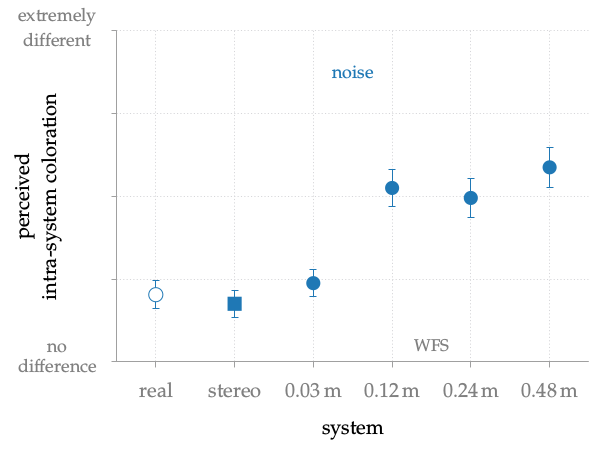
\includegraphics{fig5_06/fig5_06}
    \caption{Average results with confidence intervals for the following question:
    Is there a timbral difference between the reference and the stimulus?
    Whereby the reference and the other stimuli were presented by the same
    system each time, leading to the measurement of intra-system coloration.
    The average is calculated over all subjects and the different positions of the
    sources. All loudspeakers, including real, stereo, and WFS, were simulated
    via binaural synthesis. The results are replotted
    from~\cite[][Fig.\,8.6]{Wittek2007}.
        \reproduce{\GITHUB/fig5_06}
    }
    \label{fig:wfs_coloration_wittek}
\end{figure}

De Bruijn\autocite{DeBrujin2004} investigated the variation of
timbre for \ac{WFS} within the listening area for linear loudspeaker arrays
with different spacings.
He found large differences in terms of coloration for loudspeaker spacings of $0.5$\,m
and negligible differences for a spacing of $0.125$\,m. As source stimulus, speech shaped
noise was applied. This choice of stimulus explains why he observed less
coloration for larger spacings than Wittek.

For \ac{NFC-HOA} no results are available. For \ac{HOA} with different orders,
Solvang\sidenote[][-0.6cm]{\cite{Solvang2008}} showed that there will be stronger coloration near
the sweet-spot if too many loudspeakers are used for a given order.

In the following an experiment is described that compares the coloration of several \ac{WFS} setups and a
stereophonic setup to the reference case of a single loudspeaker.


%--%--%--%--%--%--%--%--%--%--%--%--%--%--%--%--%--%--%--%--%--%--%--%--%--%--%-
\subsection{Method}
\label{sec:coloration_method}
%

The experiment was performed with the binaural simulation method as described in
Section\,\ref{cha:binaural}. The only difference is that the dynamic
head-tracking part was disabled to exclude time-varying coloration due to head
movements.

\paragraph{Stimuli}
%
In order to ask the listeners to judge changes in timbre, a point source placed at
$(0,2.5,0)$\,m was chosen as a reference stimulus, which was realized by using a
single \ac{HRTF}. The same point source was synthesized with \ac{WFS} using
\eqref{eq:d_wfs_ps_25D} for several circular secondary source distributions.
Each distribution had the
same geometry with a radius of $3$\,m with its center at $(0,0,0)$\,m, but
different numbers of secondary sources, namely 14, 28, 56, 112, 224, 448, 896,
1\,792, 3\,584. For the distribution with 14 secondary sources, this corresponds to
a distance of $67$\,cm between the individual secondary sources going down
to $0.3$\,cm for the distribution with 3\,584 sources.
In addition, a stereophonic setup with two loudspeakers placed at $(1.4,2.5,0)$\,m
and $(-1.4,2.5,0)$\,m was included leading to a total number of 10 different
conditions, not counting the reference.
All impulse responses were normalized to the same maximum absolute amplitude
before convolving them with the audio material during the experiment.

Three different audio source materials were used.
A pulsed pink noise train composed of $800$\,ms noise bursts with $50$\,ms windowing
at the beginning and end and a pause of $500$\,ms between the bursts. This
stimulus was also used by Wittek.\autocite[][Sec.\,8.2]{Wittek2007}
As a second stimulus, a twelve second clip from the electronic song ``Luv
deluxe'' by ``Cinnamon Chasers'' was chosen. It is an instrumental song including
cymbals and subtle white noise which may help revealing coloration to a similar
degree as the pink noise stimulus does. The third stimulus was an eight second long
female speech sample.

\paragraph{Procedure}
%
The listeners were asked to rate the difference in timbre between the
reference stimulus and the other conditions on a continuous scale with
the attribute pair \emph{no difference} and \emph{very different} at its
end-points. This was accomplished with a {\small MUSHRA}
test design, including a hidden reference and a lower anchor.
The low anchor was created by high-pass
filtering the reference condition with a second order Butterworth filter with a cutoff
frequency of $5$\,kHz. The listeners were instructed to rate the
coloration and not the differences in loudness or perceived externalization of
the stimuli.
They started with one training run before the real experiment began. The
training consisted of a run with a central listening position, varying numbers of
secondary sources and a different music track.

During a single run in the experiment, the participants had to rate all
10 different conditions, the hidden
reference and the lower anchor for one given audio material.
The stimuli were looped during the experiment and the listener could
switch instantaneously between the conditions as often as she liked.
%
\begin{marginfigure}
    \centering
    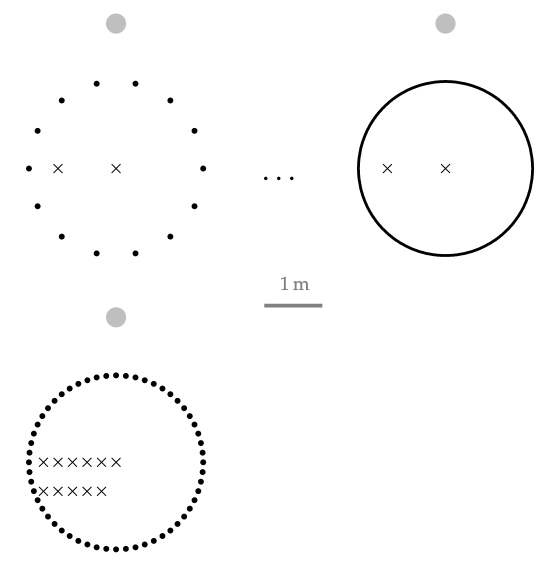
\includegraphics{fig5_07/fig5_07}
    \caption{Experimental setup for coloration experiment.
        \reproduce{\GITHUB/fig5_07}
    }
    \label{fig:wfs_coloration_setup}
\end{marginfigure}
%
The listeners were placed at two positions in the audience area, at
$(0,0,0)$\,m and $(-1,0,0)$\,m -- see Figure\,\ref{fig:wfs_coloration_setup}.
The central listening position was repeated two times, resulting in a total of
nine runs.

To investigate only the influence of the position of the listener
on coloration, another three runs were added. Here, the secondary source distribution
with 56 sources was used and
tested for the 11 different listening positions at $(0,0,0)$\,m, $(-0.25,0,0)$\,m,
$(-0.5,0,0)$\,m, $(-0.75,0,0)$\,m, $(-1,0,0)$\,m, $(-1.25,0,0)$\,m,
$(0,-0.5,0)$\,m, \linebreak
$(-0.25,-0.5,0)$\,m, $(-0.5,-0.5,0)$\,m,
$(-0.75,-0.5,0)$\,m, $(-1,-0.5,0)$\,m, $(-1.25,-0.5,0)$\,m. The head of the
listener was always orientated towards the source at all positions, to exclude a
change of the direction the synthesized source was presented from.
The synthesized point source for the listening
position at $(0,0,0)$\,m was used as the reference stimulus, which was also
included as a hidden reference. In contrast to the other runs,
no low anchor was included.

\paragraph{Participants}
%
15 normal hearing listeners were recruited for the experiment -- aged 23 to 29 years. None of
them had prior experience with psychoacoustic tests.

\paragraph{Sound Field Synthesis Settings}
%
As mentioned in
Section\,\ref{sec:spatial_aliasing_and_discrete_secondary_source_distributions},
the pre-\-equali\-zat\-ion filter in \ac{WFS} should only be applied up to the aliasing frequency.
This was done for the different secondary source setups by investigating the
amplitude spectrum at the position $(0,0,0)$\,m and adjusting the lower and
upper frequency limit of the pre-\-equali\-zat\-ion filter to create an amplitude
spectrum that is as flat as possible.
%
\begin{figure*}
    \centering
    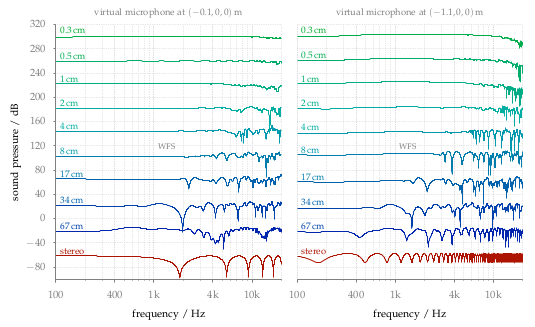
\includegraphics{fig5_08/fig5_08}
    \caption{Amplitude spectra for the varying secondary source distribution
    conditions. The spectra was simulated for the place of the left ear of
    the listener. The left graph shows the spectra
    for the central listening position, the right for the off-center position.
    The distance between the secondary sources is given for all \ac{WFS}
    spectra.
    The spectra are shifted in absolute magnitude in order to meaningfully display
    them.
    Parameters: $\xs = (0,2.5,0)$, $\xref = (0,0,0)$\,m, circular secondary
    source distribution with a diameter of $3$\,m.
        \reproduce{\GITHUB/fig5_08}
    }
    \label{fig:coloration_freq_response}
    \vspace{-0.5cm}
\end{figure*}
%
As the aliasing frequency is dependent on the listener position, the optimization
for $(0,0,0)$\,m can lead to slight deviations at other listener positions.
Figure\,\ref{fig:coloration_freq_response} shows the amplitude spectra of the
impulse responses for the different secondary source distributions synthesizing
a point source. The impulse responses were calculated for positions of the left
ear of the test participants -- excluding any \ac{HRTF}.
The calculation is identical to placing microphones
at these positions and measuring the impulse responses.
This has been done for the stereophonic setup as well.

The amplitude spectra highlight that the secondary source setup with 3\,584
sources and a corresponding distance of $0.3$\,cm between them has a more or
less flat frequency spectrum, whereas for lower numbers of secondary sources
comp-filter like deviations in the spectrum occur. The lower the number of
sources, the earlier these deviations are occurring, starting around $400$\,Hz for 
$67$\,cm.
The deviations of the amplitude spectra for the listener position
at $(-1,0,0)$\,cm tend to start at lower frequencies compared to the ones at the central
listening position.
The stereophonic amplitude spectrum has a more regular comb-filter structure due
to the involvement of only two loudspeakers. For the central position, deviations
of the spectrum in the form of large dips occur slightly below $2$\,kHz.
For the off-center listening position the deviations are spread along all
frequencies and the number of dips are more than four times as large. On the
other hand, the dips are no longer as deep as at the central position.

\begin{figure}
    \centering
    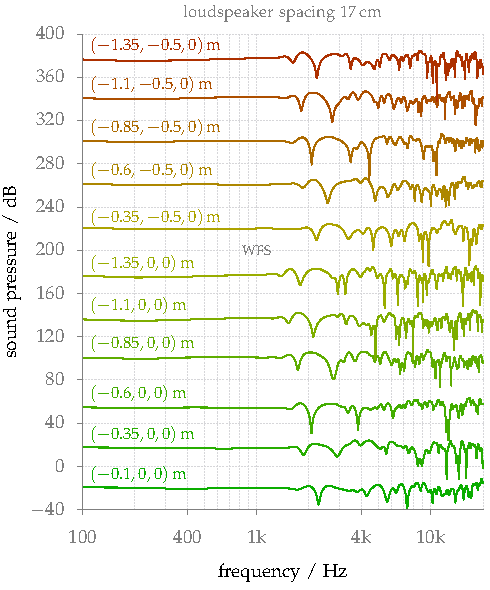
\includegraphics{fig5_09/fig5_09}
    \caption{Amplitude spectra for \ac{WFS} and a fixed secondary source
    distribution. The spectra are simulated for different positions as
    indicated by the colored labels in the figure.
    The spectra are shifted in absolute magnitude in order to display
    them.
    Parameters: $\xs = (0,2.5,0)$, $\xref = (0,0,0)$, circular secondary source
    distribution with a diameter of $3$\,m.
    \reproduce{\GITHUB/fig5_09}}
    \label{fig:coloration_freq_response_moving}
\end{figure}
%
Figure\,\ref{fig:coloration_freq_response_moving} provides an overview of the amplitude
spectra for the \ac{WFS} conditions applying a secondary source distribution
with $56$ sources and a corresponding distance of $17$\,cm between them. The
spectra are plotted for twelve different listening positions, as indicated in
the figure. The further the listener will move to the left of the audience area,
the slightly lower the spatial aliasing frequency, which is visible in the form
of an earlier start of the spectral deviations. By comparing the
first dips of the spectra it can also be observed that the dips are shifted to
higher frequencies for listener positions further to the back of the audience
area.


%--%--%--%--%--%--%--%--%--%--%--%--%--%--%--%--%--%--%--%--%--%--%--%--%--%--%-
\subsection{Results}
\label{sec:coloration_results}
%
Figure\,\ref{fig:wfs_coloration_results} summarizes the results for the nine
runs of the experiment, where the number of secondary sources was varied and the
listener was positioned at $(0,0,0)$\,m or $(-1,0,0)$\,m. Only the results for
pink noise and speech as stimuli are presented. The results for music
were only significantly ($p<0.05$)
different from the ones for
noise at two conditions, as indicated by an independent-samples Mann-Whitney U test.
%namely for the stereophonic off-center position and the central listening
%position, \ac{WFS} and a distance of $4$\,cm. For these positions the noise
%stimuli were rated as more different.
%
\begin{figure*}[t]
    \centering
    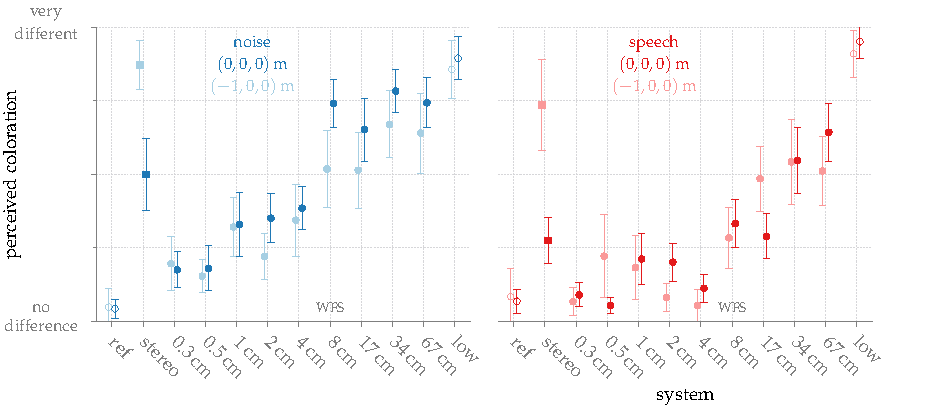
\includegraphics{fig5_10/fig5_10}
    \caption{Average results with confidence intervals for the perceived
    coloration. Dark colors show results for the central listening position,
    lighter colors for the off-center position.
        \reproduce{\GITHUB/fig5_10}
    }
    \label{fig:wfs_coloration_results}
\end{figure*}
%
The results for the two center position runs are summarized by calculating the
average for every listener before calculating the mean over all listeners. An
independent-samples Mann-Whitney U test showed that the results of the repeated
measurements were not significantly different from each other ($p<0.05$), highlighting that
the listeners were able to answer the task in a reliable way.
The test participants rated the hidden reference as not different from the
reference and the lower anchor as being very different from the reference. The overall
ratings for the \ac{WFS} stimuli show a clear dependency of the perceived
coloration on the distance between the secondary sources. The system with the lowest
distance was rated to be only slightly colored, whereas the system with the
largest inter-loudspeaker distance was rated the most colored \ac{WFS} systems. The
listener position at $(-1,0,0)$\,m exhibits a very similar pattern as the
central listening position for \ac{WFS}.
%The confidence interval is in average higher for the off-center position due to
%less measurements for this position.
For the stereophonic presentation, the perceived coloration is considerably
more dependent on
the listener position. The off-center position is rated as the most colored off
all systems. In contrast, its
perceived coloration at the central position is rated as being low to medium.
A similar coloration was achieved with an inter-loudspeaker spacing of $8$\,cm for
\ac{WFS}.

When using the speech stimuli, coloration was consistently rated lower in comparison
to the case of using noise stimuli. A \ac{WFS} system with a inter-loudspeaker
distance of $4$\,cm already achieved a transparent presentation for the speech
stimulus in terms of coloration. 

The other three runs of the experiment investigated the perceived
coloration at different positions in the audience area for a \ac{WFS} system
with 56 secondary sources with a corresponding distance
of $17$\,cm between the sources. Figure\,\ref{fig:wfs_coloration_pos} summarizes
the results.
%
\begin{figure}
    \centering
    \hspace*{0.6cm}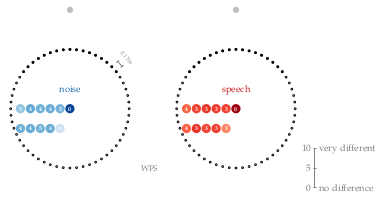
\includegraphics{fig5_11/fig5_11}
    \caption{Perceived coloration rated with the attribute pair \emph{very
    different}, \emph{no difference}. The latter corresponds to a value of $0$ in
    the figure, the former to a value of $10$. The values are written directly at
    the listening position where the listener had to rate the coloration, and are
    further highlighted by a corresponding color. The average confidence
    interval is $1.2$ over all positions.
        \reproduce{\GITHUB/fig5_11}
    }
    \label{fig:wfs_coloration_pos}
    \vspace{-0.5cm}
\end{figure}
%
The condition with the listener at the center was the hidden reference and was
not rated as being different. Most of the other positions were rated to be
equally colored, where the noise stimuli were rated to be more colored than the
other two.
Only the position at $(-0.25,-0.5,0)$\,m is
deviating from that pattern by being perceived as more colored than all other
positions.



%--%--%--%--%--%--%--%--%--%--%--%--%--%--%--%--%--%--%--%--%--%--%--%--%--%--%-
\subsection{Discussion}
\label{sec:wfs_coloration_discussion}
%
The results indicate that the number of secondary sources have a large influence
on the perceived coloration for \ac{WFS}. This is not a surprising result,
reconsidering the magnitude spectra of the different systems as shown in
Figure\,\ref{fig:coloration_freq_response}. Here, it is obvious that the spectrum
deviates from a desired flat frequency response for frequencies above the aliasing
frequency, which is directly dependent on the distance between adjacent secondary
sources.
In contrast to the localization results, where a distance of $17$\,cm already resulted
in an authentic localization accuracy, the perceived coloration never
vanishes for \ac{WFS} and pink noise as stimulus. Even for an inter-loudspeaker
spacing of $0.3$\,cm, slight coloration is perceived. 
Only for the speech stimulus and the inter-loudspeaker spacing of $0.3$\,cm the perceived
coloration was indistinguishable from the hidden reference for both the central
and off-center listening positions.

The results for stereophony suggest that sources presented by that method
exhibit coloration, meaning that binaural decoloration is not able to suppress
it completely. If the amplitude spectrum in
Figure\,\ref{fig:coloration_freq_response} is compared to the ones for \ac{WFS} it
could be concluded that the binaural decoloration has a larger impact on
stereophony, because the perceived amount of coloration seems to be less than
what may be predicted by the position of the first dip in the amplitude
spectrum.
Another possibility might be that the dips in the spectrum for stereophony are
more smeared out by the auditory filters as it is the case for \ac{WFS}.

The coloration ratings for \ac{WFS} with 56 secondary sources at
different listening positions revealed a more or less equal coloration to 
that obtained at the central listening position. However, this conclusion has to
be relativized due to the multi-dimensionality of timbre. The fact that conditions
are rated to have the same coloration compared to a reference condition does not
necessarily imply that they have no relative coloration between each other.

By averaging the coloration results for noise from
Figure\,\ref{fig:wfs_coloration_pos}, a value of $4.7$
on a scale from $0$ to $10$ is found.
This result is identical to the one Wittek\autocite{Wittek2007} obtained
for loudspeaker arrays with a distance between the loudspeaker of $12$\,cm and
$24$\,cm, which were presented in Figure\,\ref{fig:wfs_coloration_wittek}.
The distance for the 56 secondary sources in the current experiment is
$17$\,cm.

\newthought{An inspection} of the actual root mean square value of the presented signals
revealed that there were fluctuations of up to $3$\,dB between the single
conditions. Therefore, it could be that the listeners have included a
loudness-related cue in their coloration rating even if they were advised not to
do so.
To further analyze this, the correlation between the actual root mean square
values and the coloration ratings were calculated using the average for the speech
and noise stimuli, which is $0.6$ for the runs with the central listening position.
This indicates that the loudness was not the main cue for the given coloration
ratings. For the off-center listening position the correlation is $0.8$.
This highlights that the loudness could have a large contribution on the
coloration ratings for this case.
The correlation was also calculated for the conditions with different listening
positions and a fixed number of loudspeakers. When averaging over speech and
noise, the correlation results to $0.2$.
This 
indicates that the loudness did not have a major influence on the coloration ratings
for these conditions.
A more precise inspection of the listening position that was rated to be
most colored, namely $(-0.25,-0.5,0)$\,m,
nonetheless revealed that other factors could have influenced the coloration ratings.
The position $(-0.25,-0.5,0)$\,m had the loudest signal and was reported as
being less externalized compared to all other conditions by two test
participants after the experiment.

\newthought{The music and pink noise} stimuli show no significant differ- ences in all but two
positions. This indicates that even the usage of music alone might
be suitable to investigate the perceived coloration. That is of advantage,
because most listeners considered the noise stimulus as unpleasant, as revealed by
informal reports after the tests.


%--%--%--%--%--%--%--%--%--%--%--%--%--%--%--%--%--%--%--%--%--%--%--%--%--%--%-
\subsection{Conclusion}
\label{sec:coloration_conclusion}
%
The results show a clear dependency of the perceived coloration of a synthesized
point source from the given loudspeaker setup. The higher the inter-loudspeaker
spacing, the more coloration will be perceived. This direct relation is due to
the connection between the
aliasing frequency and the distance between the secondary sources. The aliasing
frequency specifies from which frequency onwards deviations in the amplitude spectrum
of the synthesized source will appear, which seems to be a good measure for the
perceived coloration of the synthesized source.

The aliasing frequency changes only to a small extent at nearby positions in the
audience area, which seems to correspond with the results showing that the perceived
coloration is similar at different positions in the audience area for \ac{WFS}
and 56 secondary sources.

For stereophony, the amount of coloration seems to be less than for a \ac{WFS}
system with a similar position of the first dip in the amplitude spectrum. This
indicates that binaural decoloration may be more pronounced for stereophony than
for \ac{WFS}.

%%%%%%%%%%%%%%%%%%%%%%%%%%%%%%%%%%%%%%%%%%%%%%%%%%%%%%%%%%%%%%%%%%%%%%%%%%%%%%%%
\section{Spectro-Temporal Artifacts}
\label{sec:spectro_temporal_artifacts}

In Section\,\ref{sec:spatial_aliasing_and_discrete_secondary_source_distributions}
the influence of discrete secondary source distributions on the perception of
synthesized sound fields was discussed. For the synthesis of focused sources
with \ac{WFS} corresponding time signals were presented in
Figure\,\ref{fig:sound_field_imp_fixed_fs}. It can be seen that for focused
sources additional wave fronts arrive at the listener position before the
desired wave front. This could have several implications for the perception of
focused sources, because the auditory system is optimized for the opposite case of
additional reflective wave fronts after a desired one, as it happens for example
in rooms.
This will be illustrated by the following example applying
a loudspeaker array and Wave Field Synthesis.

Assume the synthesis of a point source placed at $(0,1,0)$\,m
behind a linear loudspeaker array composed of 34 secondary sources with a size
of $20$\,m placed on the $x$-axis.
If an impulse is played back as audio signal through this system and
the ear signal at the right ear of a listener placed at $(4,-4,0)$\,m is recorded
it will look like the left time signal in Figure\,\ref{fig:wfs_artifacts}. The
direct sound and a bunch of early repetitions have the highest magnitude.
Later repetitions are arriving up to $50$\,ms after the first wave front, but
are lower in magnitude the later they arrive. In the upper part of the
figure the corresponding frequency response is
presented. Clear peaks and dips due to the repetitions are visible. Now
assume a system with the same magnitude spectrum, but a complete different time
pattern. This can be achieved by time reversing the impulse response as shown in
the bottom right of Figure\,\ref{fig:wfs_artifacts}. In reality this kind of
impulse responses can occur for a \ac{WFS} system synthesizing a focused source due
to the time reversing technique that is involved to achieve the desired source
model. If the impulse response from the \ac{WFS} point source is convolved
with a speech signal it adds some coloration to this signal. If the time
reversed version of the same impulse response is convolved with the same
speech signal two additional auditory events occur. One colored version of the
original one coming from another direction and an additional auditory event
consisting of spectro-temporal artifacts coming from the same direction as one of the speech
signals. The two speech signals can be downloaded and listened to via headphones
by clicking on the two \emph{listen} links.

\begin{figure*}[t]
    \centering
    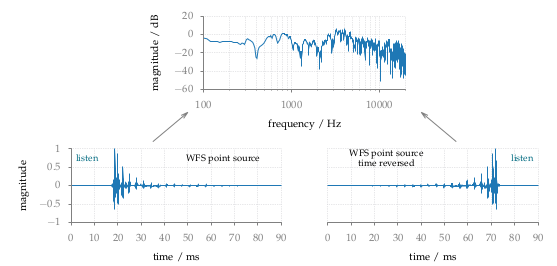
\includegraphics{fig5_12/fig5_12}
    \caption{Impulse response and amplitude spectrum of a point source
    synthesized by \ac{WFS}~\protect\eqref{eq:d_wfs_ps_25D}. Beside the impulse
    response its time reversed version is shown. Both impulse responses were
    convolved with a speech signal which can be downloaded via the \emph{listen}
    links.
    Parameters: $\xs = (0,1,0)$, $\xref = (4,-4,0)$\,m, linear secondary source
    distribution with a length of $20$\,m and 34 sources.
    \reproduce{\GITHUB/fig5_12}}
    \label{fig:wfs_artifacts}
\end{figure*}

Because the spectro-temporal artifacts are not occurring in a natural environment
and their perception is likely multi-dimensionally a first listening test was
conducted to identify important perceptual dimensions for focused sources.
A second experiment investigated the influence of the size of the secondary source
distribution on these perceptual dimensions.

%--%--%--%--%--%--%--%--%--%--%--%--%--%--%--%--%--%--%--%--%--%--%--%--%--%--%-
\subsection[Perceptual Dimensions of Focused Sources]{Experiment 1: Perceptual
Dimensions of Focused Sources in
\ac{WFS}\autocite[This experiment was done in collaboration with Matthias Geier
and parts of this section are published in][]{Geier2010a}}
\label{sec:experiment1_perceptual_dimensions_of_focused_sources_in_wfs}

To accommodate the perceptual multi-dimensionality the \ac{RGT} was used in a first
experiment to identify relevant perceptual attributes.\autocite{Kelly1955}
With this method, in a first step each participant creates her own set of
attributes and in a second step uses respective attribute scales for rating
her perception. No attributes are provided by the experimenter, and, thus,
the test subject has complete freedom in the choice of attributes.
Berg and Rumsey were the first to apply the \ac{RGT} towards perception in
spatial audio.\sidenote[][2.5cm]{\cite{Berg1999}}


%----%----%----%----%----%----%----%----%----%----%----%----%----%----%----%----
\paragraph{Stimuli}
The test was conducted via the dynamic binaural synthesis system including
binaural simulation of the secondary sources as presented in
Chapter\,\ref{cha:binaural}.
Two linear secondary source distributions with a length $L$ of $4$\,m
and $10$\,m, and a loudspeaker spacing of
$\Delta x_0 = 0.15$\,m were synthesized -- compare Figure\,\ref{fig:fs_exp1_setup}.
For the binaural simulation of the loudspeakers \acp{HRTF} of the {\small FABIAN}
manikin\sidenote[][]{\cite{Lindau2006}} measured in the anechoic chamber of Technical
University Berlin were applied.
The focused source was placed at $(0,-1,0)$\,m in front of the secondary
sources. It was synthesized with \twohalfD \ac{WFS} by applying the driving
function~\ref{eq:d_wfs_fs_25D}.
%
\begin{marginfigure}
    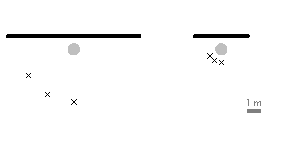
\includegraphics{fig5_13/fig5_13}
    \caption{Setup for Experiment 1. The position of the synthesized focused
    source is indicated by the grey point. The position of the listener by black
    crosses and secondary sources by black dots.
        \reproduce{\GITHUB/fig5_13}}
    \label{fig:fs_exp1_setup}
\end{marginfigure}
%

As discussed in
Section\,\ref{sec:spatial_aliasing_and_discrete_secondary_source_distributions},
the aliasing frequency
$f_\text{al}$ depends on the listener position, therefore the WFS
pre-equalisation filter was
calculated separately for each simulated listening position.
Coloration introduced by an improper choice of the
pre-equalisation filter was not part of the investigation
and should be avoided.

For both arrays, three different listener positions on a given circle around the
focused source were used. The radius was $R = 1$\,m for the short array and
$4$\,m for the long array.  Three different listener angles of $\phi =
0\degree$, $30\degree$ and $60\degree$ were applied for both array lengths -- see
Figure\,\ref{fig:fs_exp1_setup}. These result in the following six listener
positions: $(0,-2,0)$\,m, $(-0.5,-1.9,0)$\,m, $(-0.9,-1.5,0)$\,m, $(0,-5,0)$\,m,
$(-2,-4.5,0)$\,m, $(-3.5,-3,0)$\,m.
These six configurations will be referred to as $0\degree_{4\,\text{m}},
30\degree_{4\,\text{m}}, 60\degree_{4\,\text{m}}, 0\degree_{10\,\text{m}},
30\degree_{10\,\text{m}}$, $60\degree_{10\,\text{m}}$.  In all conditions, the
listener was always looking into the direction of the focused source.  A seventh,
reference condition (``ref'') was created, which consisted of a
single sound source located at the position of the focused source.
This was realized by directly using the corresponding \ac{HRTF} from the database.

As audio source signals, anechoic recordings of speech and of castanets were
chosen.\footnote{Audio examples are available as
\href{http://audio.qu.tu-berlin.de/?p=625}{\color{link}supplementary
material}.} The speech signal was an $8$\,s
sequence of three different sentences uttered by a female speaker. The
castanets recording was $7$\,s long. The levels of the stimuli were normalized to
the same loudness by informal listening for all conditions.
%The real-time convolution of these signals with the impulse responses for the
%WFS arrays was performed using the \emph{SoundScape Renderer}
%(SSR\footnote{\url{http://tu-berlin.de/?id=ssr}})~\cite{Geier2008},
%an open-source software environment for spatial
%audio reproduction.  The SSR performed a real-time convolution of
%the input signal with that
%pair of impulse responses corresponding to the instantaneous head orientation of
%the test subject as measured by a Polhemus Fastrak tracking system. In the SSR,
%switching between different audio signals is realized using a smooth cross-fade
%with raised-cosine shaped ramps.  AKG K601
%headphones were used, and the transfer functions of both earphones were
%compensated by appropriate filters~\cite{schaerer2009}.


%----%----%----%----%----%----%----%----%----%----%----%----%----%----%----%----
\paragraph{Participants}
In order to generate a large amount of meaningful attributes, test subjects with
experience in analytically listening to audio recordings were recruited.  The
experiment was conducted with 12 \emph{Tonmeister} students -- aged 21 to 33
years. The participants had between 5 years and 20 years
of musical education, and all of them had experience with listening
tests. They had normal hearing levels, and were financially compensated for
their effort.


%----%----%----%----%----%----%----%----%----%----%----%----%----%----%----%----
\paragraph{Procedure}
The participants received written instructions explaining their tasks in the two
phases of the experiment.

The \ac{RGT} procedure consisted of two parts, the \emph{elicitation phase} and
the \emph{rating phase}. In the elicitation phase, groups of three conditions
(\emph{triads}) were presented to the test subject. The subjects were able to
switch between them by pressing a corresponding button, and could listen to each
stimulus as long as they wanted.  For each triad, the subject had to decide
which two of the three stimuli were more similar, and had to describe the
characteristic which made them similar, and in which characteristic they were
different from the third stimulus (which should be the opposite of the first
property).  If there were competing aspects, only the strongest one should be
taken into account.  One attribute pair per triad had to be specified, and two
more could optionally be given if the test subject perceived several different
properties. A screenshot of the used test GUI is shown in Geier et
al.\autocite{Geier2010a}

After a short training phase, every participant had to execute this procedure 12
times, using 12 different triads.  10 of the 12 triads resulted from a complete
set of triads from the five conditions ref, $30\degree_{4\,\text{m}}$,
$60\degree_{4\,\text{m}}$, $30\degree_{10\,\text{m}}$ and
$60\degree_{10\,\text{m}}$.  The
two additional triads were $($ref, $0\degree_{4\,\text{m}}$,
$0\degree_{10\,\text{m}})$
and $(0\degree_{4\,\text{m}}$, $30\degree_{4\,\text{m}}$,
$0\degree_{10\,\text{m}})$.  These
two have been chosen in order to consider the additional, very similar
conditions together, to get attributes for the small differences between them.
Complete triads for only five conditions have been chosen because of the
time-consuming procedure -- a complete set of triads for 7 conditions would have
resulted in 35 triads.

The presented triads were the same for all participants, however, the order of
the triads and the order of conditions within a triad was alternated over all
participants based on a \emph{Latin Square} design.

After the elicitation phase, the participants took a break. During this time,
the test supervisor removed repetitions of attribute pairs for constructing the
attribute list used in the second \ac{RGT} test phase.

For this rating phase in each trial one previously elicited attribute pair was
displayed on top of the screen. Below, the seven conditions could be played back
and had to be rated on corresponding continuous sliders.
%The ratings were saved on a continuous scale ranging from $-1.0$ to $1.0$.
Once a rating was collected for
all conditions, the test subject was able to switch to the next screen, a
procedure repeated until all elicited attribute pairs were used.  Before the
actual test, a training phase had to be completed for two rating screens.

In the second session, which was in the most cases done on another day, the
elicitation and rating phase was repeated with the respective other source
stimulus. Half of the subjects were presented with the speech sample in the
first session and the castanets in the second session, and vice versa for the
other half.


%----%----%----%----%----%----%----%----%----%----%----%----%----%----%----%----
\paragraph{Results}
%
One of the main results of the experiment were the elicited attribute pairs. They
reflect the range of perceptual similarities and differences among the
conditions. Their number was different between subjects, ranging from 6 to
17 pairs for individual subjects.
The most prominent choices were artifacts (e.g. \emph{clean sound} vs.
\emph{chirpy, squeaky, unnatural sound}) and localization (\emph{left} vs.
\emph{center}). For the latter, it has to be noted that the focused source was
always positioned straight in front of
the listener. Attributes describing artifacts were provided by 10 of the 12
subjects for castanets, and by 9 subjects for speech. Localization-related
attributes were given by 7 subjects for castanets, and 5 subjects for speech.
Other common attributes were related to coloration (\emph{original} vs.
\emph{filtered}, \emph{balanced} vs. \emph{unbalanced frequency response}),
distance (\emph{far} vs. \emph{close}) and reverberation (\emph{dry} vs.
\emph{reverberant}).
All elicited attributes were originally collected in German.

The ratings of the attributes can be used to identify the underlying dimensions
which best
describe the perception of focused sources. This was done using
a \ac{PCA} for individual subjects.
For all subjects, two principal components could be identified as the main
dimensions of the perceptual space. These dimensions can explain
$90$\% of the variance for castanets and $97$\% for
speech, respectively.

\begin{figure*}[t]
    \centering
    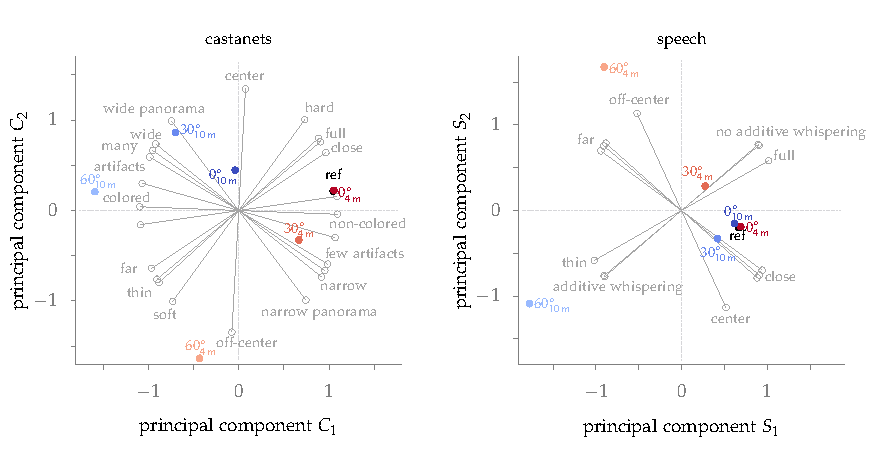
\includegraphics{fig5_14/fig5_14}
    \caption{Principal component analysis for castanets (left) and
    speech (right) for one single subject.
    The blue, red and black points indicate the position of the conditions given in the
    two-dimensional space determined by the two given components for each
    stimulus type. The gray lines show the arrangement of the attribute
    pairs in these two dimensions.
        \reproduce{\GITHUB/fig5_14}
    }
    \label{fig:pca}
\end{figure*}

This also allows to determine the positions of the different conditions in the
resulting perceptual space.  Figure\,\ref{fig:pca} shows the \ac{PCA} results
for one individual subject for the speech and castanets, respectively. The
\ac{PCA} results for another subject can be found in Geier et
al.\autocite{Geier2010a} The blue and red dots represent the different
conditions in this two-dimensional perceptual space. The gray lines show the
arrangement of elicited attribute pairs in this space.  From Figure\,\ref{fig:pca}
it can be seen that for both castanets and speech the first principal component
$C_1$ resp. $S_1$ can be interpreted as a mixture of the amount of artifacts and
the distance, and the second principal component $C_2$ resp. $S_2$ as the
localization of the source.  Considering individual conditions, it can be
observed that the $10$\,m loudspeaker array was rated to produce artifacts in
the perception of the focused source, while the artifact-related ratings for the
$4$\,m array are more or less the same as for the reference condition. For the
longer array, the amount of artifacts depends on the listener position, with the
highest rating of artifacts at the lateral position $60\degree_{10\,\text{m}}$.
The perception of a wrong direction is most distinct for the
lateral positions of the shorter array, with the condition
$60\degree_{4\,\text{m}}$ as the most prominent case.  Both lateral positions
($\phi = 60\degree$) were perceived as more off-center than the other ones.
Furthermore, it can be noted that the perceptual deviation from the reference
condition occurs for more conditions for the castanets than for the speech
stimuli.


%----%----%----%----%----%----%----%----%----%----%----%----%----%----%----%----
\paragraph{Discussion}
The results show that the amount of perceived artifacts depends on the length of
the loudspeaker array and the position of the listener, being worse for a larger
loudspeaker array and a more lateral position of the listener. This is can be
explained by the higher number of additional wave fronts for a larger
loudspeaker array and a longer time between the first additional wave front the
desired one for a lateral position. Figure\,\ref{fig:fs_direction} illustrates
this effect. There the assumption is made that every single loudspeaker
contribute an additional wave front with an amplitude that is only influenced by
the distance of the loudspeaker to the listener. The direction of incidence of
the single wave fronts is indicated by the direction the arrows point to.
The starting point on the $y$-axis of an arrow indicates the position in time
of the wave front, and the length and color of the arrow is proportional to
its amplitude in dB.
It is obvious that the larger the used
loudspeaker array, the earlier the occurrence of additional wave fronts, and the
higher their amplitude. This is due to the fact, that every single loudspeaker
adds a wave front.  For a given array, the number of wave fronts will be the
same regardless of the lateral listener position, but the time of arrival of the
first wave front will be earlier. This can be explained by the fact that the
listener is positioned closer to one end of the loudspeaker array in this case.
The loudspeakers at the ends of the array had to be driven as the first ones in
order to create a focused source in the middle of the loudspeaker array,
resulting in the significantly earlier incidence of the wave fronts from the
loudspeakers close to the listener.

\begin{figure}
    \centering
    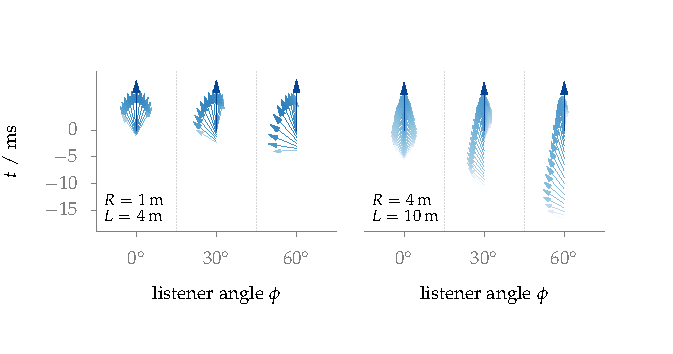
\includegraphics{fig5_15/fig5_15}
    \caption{Direction, amplitude and time of appearance of wave fronts for the
    $4$\,m loudspeaker array (left) and the $10$\,m array (right). The results
    are shown for different angles $\phi$ at a radius of $1$\,m and $4$\,m,
    respectively. The arrows are pointing towards
    the direction from which the wave fronts arrive. The
    time of appearance is given by the starting point of the arrow.
    %Note that the (temporal) starting points lie closely together for listener
    %positions close to the contributing loudspeakers of the array, and are
    %further apart when the configuration involves larger distances from the
    %loudspeakers.
    The length and color of the arrow is proportional to the amplitude of the
    wave front in dB.
    The dark blue arrows indicate the desired wave fronts.
        \reproduce{\GITHUB/fig5_15}
    }
    \label{fig:fs_direction}
    \vspace{-0.7cm}
\end{figure}

The results show a dependency of the perceived direction on the listener
position and the array size. The condition $60\degree_{4\,\text{m}}$ was perceived
as most from the left. The perceived direction can be explained by the
additional wave fronts, too.  The conditions with $\phi = 0\degree$ were
perceived from the same direction for both array lengths as the reference
condition in front of the listener. For these conditions, the additional wave
fronts have no effect on the perceived direction, because they arrive at the
listener position symmetrically from all directions -- compare
Figure\,\ref{fig:fs_direction}. For the lateral conditions, the first wave front
will come mainly from the left side of the listener. Due to the precedence effect
this can lead to localization of the sound to the direction
of the (first) wave front.
%The precedence effect can only be a first approximation to the real perception,
%because the effect is not well explored for this kind of echoes, which occur
%massive and within a time window of under $1$\,ms between each echo.
For the $10$\,m array, the perceived direction is different from that of the
shorter array.  Most of the subjects localized the sound in the same direction
as the reference.  However, a few subjects indicated that they had heard more
than one sound source -- one high-frequency chirping source from the left and a
cleaner source in front of them. This can be explained with the echo threshold
related with the precedence effect, which means that further wave fronts which
follow the first one with a lag larger than the echo threshold are perceived as
an echo.\autocite[E.g.][]{Blauert1997}

In order to verify this hypothesis, an experiment has been performed to examine
the localization dominance for this kind of time-delayed wave front
pattern.\autocite{Wierstorf2010a} Here, an approximated time of $8$\,ms between the
first wave front and the desired one has been identified to be the threshold
until which the perceived direction is dominated by the first wave front. This
is in conformance with the results for the large array.




%----%----%----%----%----%----%----%----%----%----%----%----%----%----%----%----
\subsection[Influence of the Secondary Source Geometry]{Experiment 2: Influence of the Secondary Source Geometry on the
Perception of Focused Sources in \ac{WFS}\autocite[Parts of this section are
published in][]{Wierstorf2013}}
\label{sec:fs_experiment2}

In a second experiment the main two attributes elicited in the first experiment,
namely \emph{artifacts} and \emph{direction} were investigated in more detail.
The goal of this experiment is to highlight the connection between these two
attributes and the geometry of the secondary source distribution.

As mentioned in
Chapter\,\ref{cha:sound_field_errors_and_their_perceptual_relevance}, truncation
of a sampled secondary source distribution leads to two opposite
effects. On the one hand, a smaller distribution leads to fewer additional
wave fronts and reduces the perception of artifacts as shown in the first
experiment. On the other hand, a smaller distribution is linked to stronger
diffraction of the sound field and therefore a smaller possible audience area
as well as larger focal points -- as discussed in
Figure\,\ref{fig:focal_point_size}.
In addition, the maxima and minima of the diffraction pattern could introduce
wrong \acp{ILD} and the additional wave fronts could trigger a wrong direction
due to the precedence effect.

To verify if there is an array length for which the artifacts are not audible,
and the wrong binaural cues are negligible as well, a listening test was
conducted that included three shorter array lengths together with the two
array lengths used in the first experiment.

%In the test two attribute pairs were rated by the subjects,
%one regarding the audible artifacts and one regarding the perceived position
%of the focused source.
%The middle of the array
%was again chosen at $\x = (0,0)$ in order to have a symmetric loudspeaker
%distribution around the $x$-position of the focused source.
%A more detailed discussion of the experiment is presented
%in~\cite{wierstorf2010aes}.


%----%----%----%----%----%----%----%----%----%----%----%----%----%----%----%----
\paragraph{Stimuli}
%
\begin{marginfigure}[-8cm]
    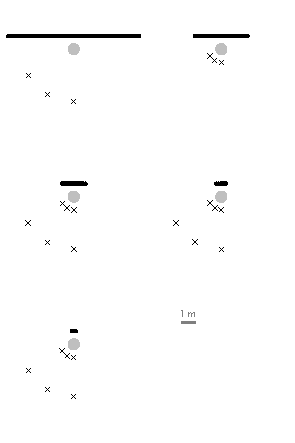
\includegraphics{fig5_16/fig5_16}
    \caption{Setup for Experiment 2. The position of the synthesized focused
    source is indicated by the grey point. The position of the listener by black
    crosses and secondary sources by black dots.
        \reproduce{\GITHUB/fig5_16}}
    \label{fig:fs_exp2_setup}
\end{marginfigure}
%
The experiment was conducted with a similar geometry and the same source materials
as described in
Section\,\ref{sec:experiment1_perceptual_dimensions_of_focused_sources_in_wfs}.
The same listener positions were used, including now the array sizes of
$L = 10$\,m, $4$\,m, $1.8$\,m, $0.75$\,m and $0.3$\,m.
For the three shortest arrays the listener were placed at all six positions.
Figure\,\ref{fig:fs_exp2_setup} summarizes the experimental
setup.\sidenote[][-1.5cm]{Audio
examples are available as
\href{http://audio.qu.tu-berlin.de/?p=625}{\color{link}supplementary material}.}


%----%----%----%----%----%----%----%----%----%----%----%----%----%----%----%----
\paragraph{Participants}
Six test subjects participated in the test. All of them were members of
the Audio Group at {\small TU} Berlin and were normal hearing.


%----%----%----%----%----%----%----%----%----%----%----%----%----%----%----%----
\paragraph{Procedure}
After an introduction and a short training phase with a violin piece as source
material, one half of the participants started the first session
presenting speech, the other half presenting castanets.
In a second session, the speech and castanets source materials were switched
between the groups. The subjects were presented with a screen
containing nine sliders representing nine different conditions.
At the top of the screen, one of the two attribute pairs  \emph{few artifacts}
vs. \emph{many artifacts} and \emph{left} vs. \emph{right} were presented.
After a subject had rated all conditions, the next
attribute pair was presented for the same conditions.
Thereby the order of the
conditions attached to the slider and the appearance of the
attribute pairs was randomized. This procedure was repeated
three times, once for all the array conditions assessed in case of each
listening angle $\phi$.
For the listening angle of $0\degree$, the attribute pair
\emph{left} vs. \emph{right} was omitted.


%----%----%----%----%----%----%----%----%----%----%----%----%----%----%----%----
\paragraph{Results}
\begin{figure}
    \centering
    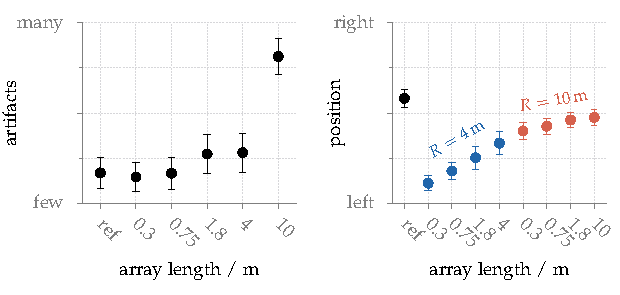
\includegraphics{fig5_17/fig5_17}
    \caption{Mean and standard error for the
        rating of the attribute pair \emph{few artifacts} vs. \emph{many
        artifacts} plotted over the condition.
        The mean is calculated over all subjects,
        source materials and the different listener positions.
        \reproduce{\GITHUB/fig5_17}
    }
    \label{fig:fs_exp2_results}
\end{figure}
%
The left part of Figure\,\ref{fig:fs_exp2_results} presents the mean ratings
over all subjects, all listener positions and both source materials (speech and
castanets) for the attribute pair \emph{few artifacts} vs. \emph{many
artifacts}.  Hence, the only independent variable is the length of the secondary
source distribution plotted on the $x$-axis.
The $0\degree$ position for the speech material
resulted as an outlier, and was not considered for the plot.  At this position
and with speech as source material, artifacts are only little audible.  On the
other hand, there is the coloration introduced by the spatial sampling, and
independent of the fact that focused sources were realized. An interview with
the subjects revealed, that four of them have rated this coloration rather than
the targeted audible artifacts.  It can be seen in the figure that the results
for the different loudspeaker arrays build three different groups.  The two
shortest arrays resulted in as few artifacts as the reference condition.  The
$10$\,m array was found to lead to strong artifacts, as it was expected from the
previous experiment. The amount of artifacts caused by the $1.8$\,m and the
$4$\,m array are positioned between these two groups.  A one-way ANOVA shows
that the mentioned three groups are statistically different ($p < 0.05$) from
each other, and not different within each group.

In the right part of Figure\,\ref{fig:fs_exp2_results}, the results for the
attribute pair \emph{left} vs. \emph{right} are presented. The means for
the arrays were calculated over the $30\degree$ and $60\degree$ conditions,
but once for each radius indicated by the two different shades of gray. For a
listener angle of $0\degree$ the rating of this attribute pair was omitted.
It can be seen that the reference condition (arriving from straight ahead
of the listener) was rated to come slightly from the right side. All other
conditions came from the left side, where shorter arrays and smaller radii
lead to a rating further to the left.

The two different source materials speech and castanets showed significant
differences only for the $10$\,m array and the $30\degree$ and $60\degree$
positions, with more artifacts perceivable for the castanets stimuli.


%----%----%----%----%----%----%----%----%----%----%----%----%----%----%----%----
\paragraph{Discussion}
As shown already in the first experiment, the appearance of additional wave
fronts due to spatial aliasing leads to strong artifacts for focused sources.
The arrival time of the first wave front at the
listener position can be reduced by using a shorter loudspeaker array.  This
leads to a reduction of audible artifacts, as shown by the results for the
attribute pair \emph{few artifacts} vs. \emph{many artifacts}.  The two smallest
arrays with a length of $0.3$\,m and $0.75$\,m are rated to have the same amount
of artifacts as the single loudspeaker reference.

All three loudspeaker arrays with a length of $L<2$\,m have arrival times of the
first wave front of below $5$\,ms. This means that they fall in a time window in
which the precedence effect should work, and no echo should be audible.  The
artifacts audible for the array with $L = 1.8$\,m are therefore due to a
comb-filter shaped ripple in the frequency spectrum of the signal, as a result
of the temporal delay and superposition procedure of the loudspeakers,
see~\eqref{eq:d_wfs_fs_25D}.

However, there are other problems related with a shorter array.  The main
problem is the localization of the focused source.
Figure\,\ref{fig:fs_exp2_results} shows a relation between array length
and localization: the shorter the array, the further left the focused source
is perceived.  This result implies that the precedence effect cannot be the only
reason for the wrong perception of the location. For a shorter array, too, the
first wave front arrives from the loudspeaker at the edge of the array. This
loudspeaker will be positioned less far to the left for a shorter array than for
a longer array.  Therefore, it is likely that the diffraction due to the short
array length introduces wrong binaural cues, namely a wrong ILD.


%--%--%--%--%--%--%--%--%--%--%--%--%--%--%--%--%--%--%--%--%--%--%--%--%--%--%-
\subsection{Conclusion}
\label{sec:fs_conclusion}

Sound field synthesis allows for the synthesis of focused sources
placed directly in the audience area, a feature that makes it distinct from all
stereophonic presentation techniques. The problematic aspect of focused sources
is that the additional wave fronts due to spatial sampling appear not after but
before the desired wave front. This is inherent for focused sources due to the
time reversal technique employed to create them.

Experiments were carried out that investigated the influence of these special
situation in the perception of focused sources. For loudspeaker arrays larger
than $2$\,m spectro-temporal artifacts were perceivable in addition to
coloration of the synthesized source. By applying smaller arrays or smaller
parts of a large array these artifacts can be eliminated. On the other hand
by using smaller arrays the localization of the focused source is impaired.
